\section{Modelo conceptual}
A continuacion presentaremos un diagrama de conceptos que pretende modelar los principales conceptos visibles en nuestra soluci�n. El mismo pretende brindar una visi�n completa de lo que el sistema puede observar

\begin{landscape}
\subsection{Diagrama}
\begin{figure}[H]
\centering
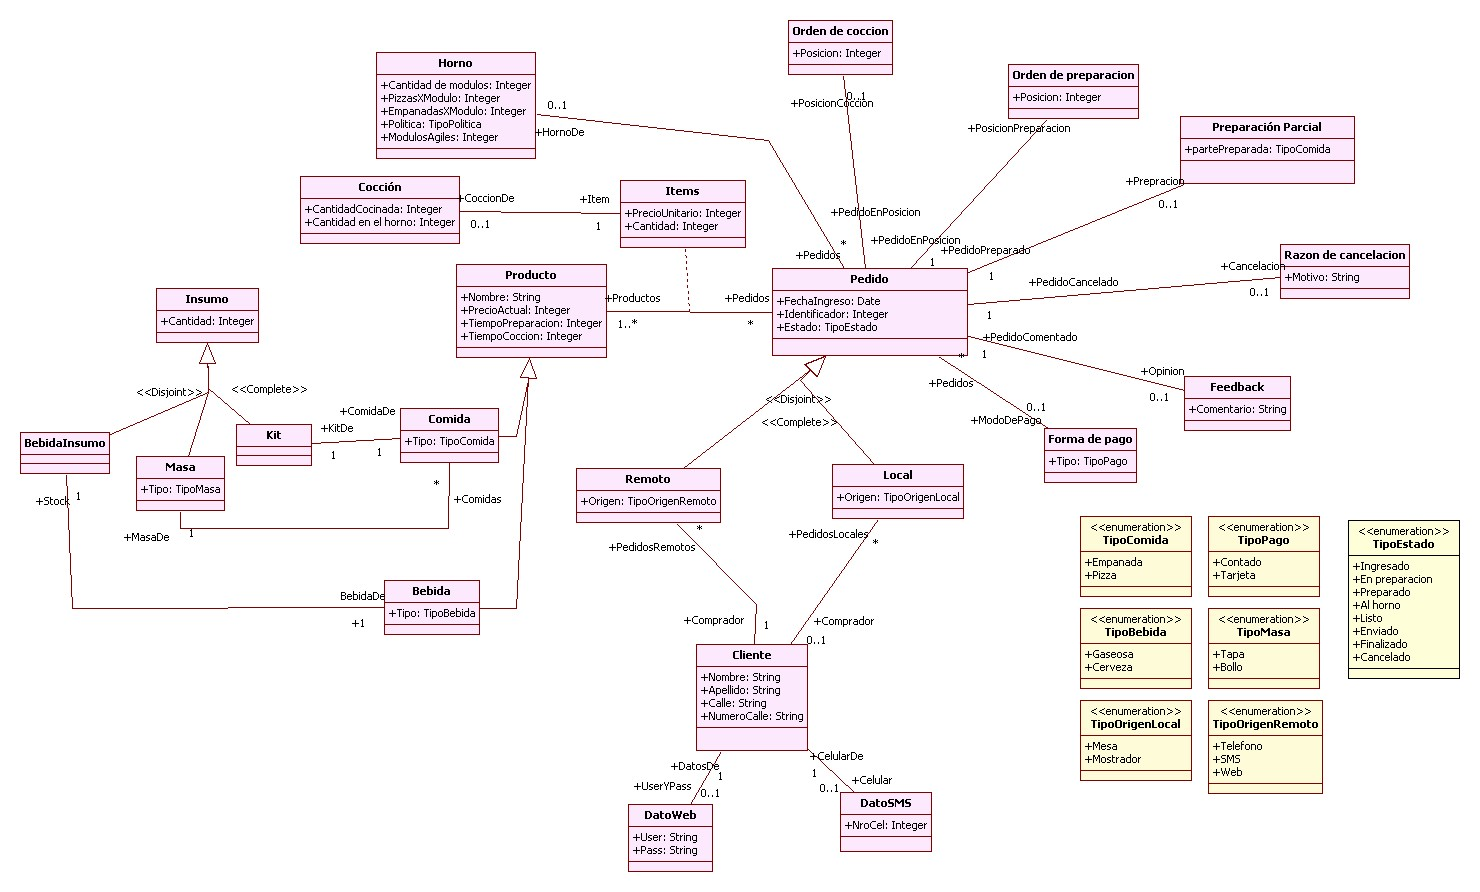
\includegraphics[scale=.5]{conceptos}
\end{figure}
\end{landscape}
%TODO: controlar esta descripci�n.
En el diagrama lo que observamos primeramente es que los pedidos son el concepto principal. Un pedido tiene una fecha de ingreso, un identificador unico en el sistema, y un estado. El pedido esta asociado a varios productos (Pizzas de muzzarella, napolitana, empanadas de carne, coca cola), y lleva una cierta cantidad de cada uno de ellos. Ademas estos productos se ligaron al pedido con un precio particular, que no necesariamente es el precio actual ya que los precios pueden cambiar.
Segun el estado que posea un pedido, esta relacionado con diferentes clases conceptuales. Por ejemplo un pedido cancelado, tiene una razon de cancelaci�n, un pedido ingresado tiene un orden en la cola de ingreso de pedidos a la cocina, el cual determina cuando pasa a ser preparado; una preparaci�n parcial esta relacionado con un pedido mixto que posee alguno de sus subproductos (pizzas o empanadas) ya preparados.

Los productos pueden ser comida (pizzas o empanadas) o bebidas. Para cada uno de ellos el sistema controla la cantidad disponible de insumos, en el caso de la comida es masa y kit, mientras que en el caso de las bebidas es la cantidad de bebidas en stock.

Los pedidos pueden ser locales o remotos segun su origen. Los pedidos remotos siempre tienen asociados a un cliente registrado, en cambio los pedidos locales podr�an estar vinculados a un cliente cuyos datos son desconocidos, por eso podemos considerar que pueden estar vinculados a 0 clientes. Un pedio remoto tiene necesariamente un forma de pago vinculada, mientras que un pedido local puede no tenerla, ya que si el cliente esta en una mesa, la forma de pago se decide cuando el cliente este dispuesto a pagar.

Un cliente registrado tiene cierta informaci�n basica, pero ademas puede registrar en alg�n momento otra informaci�n extra que lo habilita a hacer pedidos web, o pedidos SMS.

Cuando un pedido esta cocinandose, algunos de sus items estan en el horno, otros ya fueron cocinados. Esta informaci�n se encuentra en la clase cocci�n relacionada con los items de un producto.

Un pedido tiene uno o cero hornos porque el pedido podria ser exclusivamente de bebidas.
\subsection{Diccionario de datos} %TODO: no se q es

\subsection{Restricciones al MC en OCL}
\restr{Un pedido tiene un conjunto de estados valido}{}
\restr{Un pedido llega a los estado en orden valido}{}
\restr{Si el pedido no era en el local o ya fue entregado, entonces tiene una forma de pago}{}
\restr{Forma de pago tarjeta si y solo si pedido local o web}{}
\restr{Cliente tiene pedidos remotos web si tiene datos web y remotos sms si tiene numero de celular}{}
\restr{Si el pedido tiene solo pizzas y se esta preparando, empanadaspreparadas es true}{}
\restr{Si el pedido tiene solo empanadas y se esta preparando, pizzaspreparadas es true}{}
\restr{Un pedido tiene feedback si era remoto}{}
\restr{Cada estado se relaciona con un estado-pedido adecuado}{}
\restr{Todos los datos web son diferentes}{}
%TODO: q onda con los numeros?
\restr{Todos los numeros de celular son diferentes}{}
\restr{Todos los numeros de telefono son diferentes}{}
%TODO: dudoso
\restr{Para los pedidos de la misma fecha, los precios de sus items son iguales}{}
\restr{Un pedido tiene un horno si y solo si no es de solo bebidas}{}
\restr{Hay solo siete estados y tienen los nombres de los estados de pedido}{}
\restr{No hay dos pedidos con el mismo identificador}{}
\restr{}{}